\documentclass[wcp]{jmlr}

\usepackage[nolist]{acronym}
\usepackage{algorithm,algorithmic}
\usepackage{times}
\usepackage{enumerate}

\DeclareMathOperator*{\Exp}{\mathbf{E}}
\DeclareMathOperator{\Regret}{Regret}
\DeclareMathOperator{\Wealth}{Wealth}
\DeclareMathOperator{\Reward}{Reward}
\DeclareMathOperator{\polylog}{polylog}

\newcommand{\N}{\mathbb{N}}     % natural numbers
\newcommand{\R}{\mathbb{R}}     % real numbers
\newcommand{\C}{\mathbb{C}}     % complex numbers
\renewcommand{\H}{\mathcal{H}}  % Hilbert space
\newcommand{\KL}[2]{D\left({#1}\middle\|{#2}\right)}  % KL divergence
\newcommand{\norm}[1]{\left\|{#1}\right\|}
\DeclareMathOperator*{\argmin}{arg\,min}
\DeclareMathOperator*{\argmax}{arg\,max}
\newcommand{\indicator}{\mathbf{1}}
\newcommand{\scO}{\mathcal{O}}  % big-Oh

\begin{acronym}
\acro{EG}{Exponentiated Gradient}
\acro{DFEG}{Dimension-Free Exponentiated Gradient}
\acro{OMD}{Online Mirror Descent}
\acro{ASGD}{Averaged Stochastic Gradient Descent}
\acro{OGD}{Online Gradient Descent}
\acro{SGD}{Stochastic Gradient Descent}
\acro{PiSTOL}{Parameter-free STOchastic Learning}
\acro{OCO}{Online Convex Optimization}
\acro{OLO}{Online Linear Optimization}
\acro{RKHS}{Reproducing Kernel Hilbert Space}
\acro{IID}{Independent and Identically Distributed}
\acro{SVM}{Support Vector Machine}
\acro{ERM}{Empirical Risk Minimization}
\acro{COCOB}{Continous Coin Betting}
\acro{MBA}{Master Betting Algorithm}
\acro{KT}{Krichevsky-Trofimov}
\acro{LEA}{Learning with Expert Advice}
\acro{FTRL}{Follow The Regularized Leader}
\end{acronym}


\jmlrvolume{1}
\jmlryear{2016}
\jmlrworkshop{ICML 2016 AutoML Workshop}

\author{%
\Name{Francesco Orabona}
\Email{francesco@orabona.com}
\AND
\Name{D\'avid P\'al}
\Email{dpal@yahoo-inc.com}\\
\addr Yahoo Research, New York}

\title{Parameter-Free Convex Learning through Coin Betting}

\begin{document}

\maketitle

\begin{abstract}
We present a new parameter-free algorithm for online linear optimization over a Hilbert space. It is theoretically optimal, with regret guarantees as good as with the best possible learning rate. The algorithm is simple and easy to implement. The analysis is given via the adversarial coin-betting game, Kelly betting and the Krichevsky-Trofimov
estimator. Applications to obtain parameter-free convex optimization and machine learning algorithms are shown.
\end{abstract}

\section{Introduction}
\label{section:introduction}

We consider the \ac{OLO}~\cite{Cesa-Bianchi-Lugosi-2006, Shalev-Shwartz-2011}
setting. In each round $t$, an algorithm chooses a point $w_t$ from a convex
\emph{decision set} $K$ and then receives a reward vector $g_t$. Algorithm's
goal is to keep its \emph{regret} small, defined as the difference between its
cumulative reward and the cumulative reward of a fixed strategy $u \in K$, that
is
\[
\Regret_T(u) = \sum_{t=1}^T \langle g_t, u \rangle - \sum_{t=1}^T \langle g_t, w_t \rangle \; .
\]

We focus on two particular sets, the $N$-dimensional probability simplex
$\Delta_N = \{ x \in \R^N ~:~ x \ge 0, \norm{x}_1 = 1\}$ and the Hilbert space
$\H$.  \ac{OLO} over $\Delta_N$ is referred to as the problem of \ac{LEA}.  We
assume bounds on the norms of the reward vectors: For \ac{OLO} over $\H$, we
assume that $\norm{g_t} \le 1$, and for \ac{LEA} we assume that $g_t \in
[0,1]^N$.

\ac{OLO} is a basic building block of many machine learning problems. For
example, \ac{OCO}, the problem analogous to \ac{OLO} where $-\langle g_t, w_t
\rangle$ is generalized to $\ell_t(w_t)$ where $\ell_t$ is an arbitrary convex
function, is solved through a reduction to an
\ac{OLO}~\cite{Shalev-Shwartz-2011}.  \ac{LEA}~\cite{Littlestone-Warmuth-1994,
Vovk-1998, Cesa-Bianchi-Freund-Haussler-Helmbold-Schapire-Warmuth-1997}
provides a way of combining classifiers and it is at the heart of
boosting~\cite{Freund-Schapire-1997}. Batch and stochastic convex optimization
can be solved through a reduction to \ac{OLO}~\cite{Shalev-Shwartz-2011}.
Statistical learning with convex losses can also seen as stochastic convex
optimization and solved through \ac{OCO}~\cite{Munro-1951}, that in turns can
be reduced to \ac{OLO}.

However, to achieve small regret, most of the algorithms still require to set
hyperparameters (e.g., learning rates, regularization weights) in order to
achieve the best possible theoretical and empirical performance.  Recently, a
new family of parameter-free algorithms that has been proposed, both for
\ac{LEA}~\cite{Chaudhuri-Freund-Hsu-2009, Chernov-Vovk-2010, Luo-Schapire-2014,
Luo-Schapire-2015, Koolen-van-Erven-2015} and for \ac{OLO}/\ac{OCO} over
Hilbert spaces~\cite{Streeter-McMahan-2012, Orabona-2013,
McMahan-Abernethy-2013, McMahan-Orabona-2014, Orabona-2014}.  These algorithms
adapt to the number of experts and to the norm of the optimal predictor,
respectively, without the need to tune parameters.  Surprisingly, these two
families of algorithms are very similar as shown in the non-constructive
framework of~\cite{Foster-Rakhlin-Sridharan-2015}.  Given the connections
between \ac{OLO}/\ac{LEA} and machine learning, these algorithms allow to
design parameter-free batch machine learning algorithms through straightforward
reductions~\cite{Orabona-2014, Luo-Schapire-2015}.  Yet, all of existing
algorithms for LEA either have sub-optimal regret bound (e.g. extra $\scO(\log
\log T)$ factor) or sub-optimal running time (e.g. requiring solving a
numerical problem in every round, or with extra factors); see
Table~\ref{table:bounds}.

\textbf{Contributions.} We show that a more fundamental notion subsumes \emph{both}
\ac{OLO} and \ac{LEA} parameter-free algorithms. We show that the ability to
maximize the wealth in bets on the outcomes of coin flips \emph{implies}
\ac{OLO} and \ac{LEA} parameter-free algorithms.  Hence, we present a novel
framework to characterize betting algorithms through potential functions and we
instantiate it with the Krichevsky-Trofimov estimator.  The resulting
algorithms are new, simple, and natural. They also have optimal guarantees on
time and regret, see Table~\ref{table:bounds}.

\begin{table}
\begin{center}
\resizebox{\linewidth}{!}{%
\begin{tabular}{l c c c c}
\toprule
Algorithm & Worst-case regret guarantee& \begin{tabular}{@{}c@{}}Per-Round Time\\Complexity\end{tabular} & Adaptive & \begin{tabular}{@{}c@{}}Unified \\  design\end{tabular}\\
\midrule
\cite{Abernethy-Bartlett-Rakhlin-Tewari-2008} & \begin{tabular}{@{}c@{}}$U \sqrt{T}$ for any $u \in \H$ s.t. $\norm{u} \le U$\\
$\scO(T)$ otherwise\end{tabular} & $\scO(1)$ &  \\
OGD, $\eta=\tfrac{1}{\sqrt{T}}$ \cite{Shalev-Shwartz-2011} & $\scO((1 + \norm{u}^2)\sqrt{T})$, $\forall u \in \H$ & $\scO(1)$ &  \\
\cite{McMahan-Orabona-2014} & $\scO(\norm{u}\sqrt{T \ln(1+\norm{u}T)})$, $\forall u \in \H$ & $\scO(1)$ & \checkmark \\
This paper, Sec.~\ref{section:kt-olo} & $\scO(\norm{u}\sqrt{T \ln(1+\norm{u}T)})$, $\forall u \in \H$ & $\scO(1)$ & \checkmark & \checkmark\\
\midrule
Hegde~\cite{Freund-Schapire-1997}, $\eta=\sqrt{\tfrac{\ln N - U}{T}}$ & $\scO\left(\sqrt{T (\ln N -U)}\right)$ for any $u \in \Delta_N$ s.t. $H(u) \geq U$ & $\scO(N)$ &  \\
\cite{Chaudhuri-Freund-Hsu-2009}  & $\scO\left(\sqrt{T \KL{u}{\tfrac{1}{N}\boldsymbol{1}}}+\ln^2 N\right)$, $\forall u \in \Delta_N$ & $\scO(N\,K)$\footnotemark[1]& \checkmark \\
\cite{Chernov-Vovk-2010} & $\scO\left(\sqrt{T \left(1+\KL{u}{\tfrac{1}{N}\boldsymbol{1}}\right)}\right)$, $\forall u \in \Delta_N$ & $\scO(N\,K)$\footnotemark[1] & \checkmark \\
\cite{Chernov-Vovk-2010, Luo-Schapire-2015,Koolen-van-Erven-2015} & $\scO\left(\sqrt{T \left(\ln \ln T+\KL{u}{\tfrac{1}{N}\boldsymbol{1}}\right)}\right)$, $\forall u \in \Delta_N$ & $\scO(N)$ & \checkmark \\
\cite{Foster-Rakhlin-Sridharan-2015} & $\scO\left(\sqrt{T \left(1+\KL{u}{\tfrac{1}{N}\boldsymbol{1}}\right)}\right)$, $\forall u \in \Delta_N$ & $\scO(N \max_{u \in \Delta_N} \ln \KL{u}{\pi})$\footnotemark[2] & \checkmark & \checkmark \\
This paper, Sec.~\ref{section:kt-lea} & $\scO\left(\sqrt{T \left(1+\KL{u}{\tfrac{1}{N}\boldsymbol{1}}\right)}\right)$, $\forall u \in \Delta_N$ & $\scO(N)$ & \checkmark & \checkmark\\
\bottomrule
\end{tabular}}
\caption{Algorithms for \ac{OLO} over Hilbert space and \ac{LEA}}
\label{table:bounds}
\end{center}
\end{table}
\footnotetext[1]{These algorithms require to solve a numerical problem at each step. The number $K$ is the number of steps needed to reach the required precision. Neither the required precision
nor the number of steps to reach it is calculated in these papers. In general, $K$ is a function of the number rounds $T$ and the number of experts $N$.}
\footnotetext[2]{A slighly modified version of algorithm in \cite{Foster-Rakhlin-Sridharan-2015} can be implemented with the stated time complexity~\cite{Foster:private}.}

\section{How to Tune the Learning Rates?}
\label{section:learning-rates}

Consider \ac{OLO} over a Hilbert Space $\H$. \ac{OGD} with learning rate
$\eta$ satisfies~\citep{Shalev-Shwartz-2011}
\begin{equation}
\label{equation:ftrl-vanila}
\forall u \in \H \qquad \Regret_T(u) \le \tfrac{\norm{u}^2}{2\eta} + \tfrac{\eta T}{2} \; .
\end{equation}
It is obvious that the optimal tuning of the learning rate depends on the
unknown norm of $u$.

The simple choice $\eta = 1/\sqrt{T}$ leads to an algorithm that satisfies
\begin{equation}
\label{equation:ftrl-vanila-2}
\Regret_T(u) \le \tfrac{1}{2}\left(1+\norm{u}^2\right)\sqrt{T} \; .
\end{equation}
However, in this bound the dependency on $\norm{u}$ is suboptimal: The
quadratic dependency can be replaced by an (almost) linear dependency.
Starting from \eqref{equation:ftrl-vanila}, if we choose the learning rate
$\eta = D/\sqrt{T}$, we get a family of algorithms parametrized by $D \in
[0,\infty)$ that satisfy
\begin{equation}
\label{equation:ftrl-vanila-3}
\forall u \in \H : \norm{u} \le D \quad  \Longrightarrow \quad \Regret_T(u) \le D \sqrt{T} \; .
\end{equation}
Instead of a family of algorithms parametrized by $D \in [0,\infty)$ satisfying
the bound \eqref{equation:ftrl-vanila-3}, one \emph{would like
to have} a single algorithm (without any tuning parameters) satisfying
\begin{equation}
\label{equation:olo-parameter-free}
\forall u \in \H \qquad \Regret_T(u) \le \norm{u} \sqrt{T} \; .
\end{equation}
Notice that \eqref{equation:olo-parameter-free} is stronger than
\eqref{equation:ftrl-vanila-3} in the following sense: A single algorithm
satisfying \eqref{equation:olo-parameter-free} implies
\eqref{equation:ftrl-vanila-3} for all values of $D \in [0,\infty)$. However,
a family of algorithms $\{A_D : D \in [0,\infty)\}$ parametrized by $D$ where
$A_D$ satisfies \eqref{equation:ftrl-vanila-3}, does not yield a single
algorithm that satisfies \eqref{equation:olo-parameter-free}.  Finally, note
that \eqref{equation:olo-parameter-free} has better dependency on $\norm{u}$
than \eqref{equation:ftrl-vanila-2}.

There have been a lot of work on algorithms \citep{Streeter-McMahan-2012,
Orabona-2013, McMahan-Abernethy-2013,
McMahan-Orabona-2014,Orabona-Pal-2016-parameter-free} that satisfy a slightly
weaker version of \eqref{equation:olo-parameter-free}. Namely, their regret satisfies
\begin{equation}
\label{equation:olo-parameter-free-2}
\forall u \in \H \qquad \Regret_T(u) \le \big(O(1)+\polylog(1 + \norm{u})\norm{u} \big) \sqrt{T} \; .
\end{equation}
It can be shown that for \ac{OLO} over Hilbert space the extra poly-logarithmic
factor is necessary~\citep{McMahan-Abernethy-2013,Orabona-2013}. Algorithms
satisfying \eqref{equation:olo-parameter-free-2} are called
\emph{parameter-free}, since they do not need to know $D$, yet they have an
optimal dependency on $\norm{u}$.

\section{Parameter-Free Algorithms}


\begin{algorithm}[t]
\caption{Algorithm for OLO over Hilbert space $\H$
\label{algorithm:hilbert-space-olo}}
\begin{algorithmic}[1]
{
\FOR{$t=1,2,\dots$}
\STATE{Predict with $x_t \leftarrow - \frac{1}{t} \left(1 - \sum_{i=1}^{t-1} \langle \ell_i, x_i \rangle \right) \sum_{i=1}^{t-1} \ell_i$}
\STATE{Receive loss vector $\ell_t \in \H$ such that $\norm{\ell_t} \le 1$}
\ENDFOR
}
\end{algorithmic}
\end{algorithm}
\begin{algorithm}[t]
\begin{algorithmic}[1]
\caption{Algorithm for Learning with Expert Advice \label{algorithm:experts}}
{
\REQUIRE{Number of experts $N$, number of rounds $T$, prior distribution $\pi \in \Delta_N$}
\FOR{$t=1,2,\dots,T$}
\STATE{For each $i \in [N]$, set $w_{t,i} \leftarrow \tfrac{\sum_{j=1}^{t-1} g_{j,i}}{t+T/2} \left(1 + \sum_{j=1}^{t-1} g_{j,i} w_{j,i} \right)$ and $\widehat{p}_{t,i} \leftarrow \pi_i [w_{t,i}]_+$}
\STATE{Predict with $p_t \leftarrow
\begin{cases}
\widehat{p}_t/\norm{\widehat{p_t}}_1 & \text{if $\norm{\widehat p_t}_1 > 0$} \\
\pi & \text{if $\norm{\widehat p_t}_1 = 0$}
\end{cases}$}
\STATE{Receive loss vector $\ell_t \in [0,1]^N$}
\STATE{For each $i \in [N]$, set $g_{t,i} \leftarrow \begin{cases}
\langle \ell_t, p_t \rangle - \ell_{t,i} & \text{if $w_{t,i} > 0$} \\
[\langle \ell_t, p_t \rangle - \ell_{t,i}]_+ & \text{if $w_{t,i} \le 0$}
\end{cases}$}
\ENDFOR
}
\end{algorithmic}
\end{algorithm}

We present algorithms for \ac{OLO} over real Hilbert space $\H$
(Algorithm~\ref{algorithm:hilbert-space-olo}) and
\ac{LEA}~(Algorithm~\ref{algorithm:experts}).  The theorems below upper bound
their regret, the proofs can be found in~\cite{Orabona-Pal-2016-parameter-free}.

\begin{theorem}[Regret Bound for Algorithm~\ref{algorithm:hilbert-space-olo}]
\label{theorem:hilbert-space-olo-regret}
Let $\{\ell_t\}_{t=1}^\infty$ be any sequence of loss vectors
in a Hilbert space $\H$ such that $\norm{\ell_t} \le 1$.
Algorithm~\ref{algorithm:hilbert-space-olo} satisfies
$$
\forall \, T \ge 0 \quad
\forall u \in \H \qquad \qquad
\Regret_T(u) \le \norm{u} \sqrt{T \ln\left(1 + 4T^2 \norm{u}^2 \right)} + 1 \;.
$$
\end{theorem}

\begin{theorem}[Regret Bound for Algorithm~\ref{algorithm:experts}]
\label{theorem:experts-regret}
Let $N \ge 2$ and $T \ge 0$ be integers. Let $\pi \in \Delta_N$ be a prior.
For any sequence $\ell_1, \ell_2, \dots, \ell_T \in
[0,1]^N$ of loss vectors, Algorithm~\ref{algorithm:experts}
satisfies
$$
\forall u \in \Delta_N \qquad \qquad \Regret_T(u) \le \sqrt{3T (4 + \KL{u}{\pi})} \; .
$$
\end{theorem}

Note that, the requirement of knowing the number of rounds $T$ in Algorithm~\ref{algorithm:experts} can be lifted by
the standard doubling trick, again in a parameter-free way; for details
see~\cite{Orabona-Pal-2016-parameter-free}.



\section{Design and Analysis of Algorithms}

Algorithm~\ref{algorithm:hilbert-space-olo}
is based on the adversarial coin-betting problem.

\textbf{Adversarial Coin Betting.}
Consider a gambler making repeated bets on the outcomes of adversarial coin
flips. The gambler starts with an initial endowment of $1$ dollar. In each
round $t$, he bets on the outcome of a coin flip $g_t \in \{-1,1\}$, where $+1$
denotes heads and $-1$ denotes tails.  The outcome $g_t$ is chosen by an
adversary.  The gambler can bet any amount on either heads or tails. However,
he cannot borrow any additional money. If he loses, he loses the betted amount;
if he wins, he gets the betted amount back and, in addition to that, he gets
the same amount as a reward.  We encode the gambler's bet in round $t$ by a
single number $\beta_t \in [-1,1]$. The sign of $\beta_t$ encodes whether he is
betting on heads or tails. The absolute value encodes the betted amount as the
fraction of his current wealth.  Let $\Wealth_t$ be gambler's wealth at the end
of round $t$. It satisfies
\begin{align}
\label{equation:wealth-recurrence}
\Wealth_0 & = 1 &
& \text{and} &
\Wealth_t & = (1 + g_t \beta_t) \Wealth_{t-1} \qquad \text{for $t \ge 1$} \; .
\end{align}
Note that since $\beta_t \in [-1,1]$, gambler's wealth stays always
non-negative.

\textbf{Kelly Betting and Krichevsky-Trofimov Estimator.}
For sequential betting on i.i.d. coin flips, the optimal strategy has been
proposed by \citet{Kelly-1956}.  The strategy assumes that the coin flips
$\{g_t\}_{t=1}^\infty$, $g_t \in \{+1,-1\}$, are generated i.i.d. with known
probability of heads. If $p \in [0,1]$ is the probability of heads, the Kelly
bet is $\beta_t = 2p - 1$. He showed that, in the long run, this strategy will
provide more wealth than betting any other fixed fraction~\cite{Kelly-1956}.

For adversarial coins, Kelly betting does not make sense.
\citet{Krichevsky-Trofimov-1981} proposed to replace $p$ with an estimate:
After seeing coin flips $g_1, g_2, \dots, g_{t-1}$, use the empirical
estimate $k_t = \frac{1/2 + \sum_{i=1}^{t-1} \indicator[g_i = +1]}{t}$. Their
estimate is commonly called \emph{KT estimator}\footnote{Compared to the
standard maximum likelihood estimate $\frac{\sum_{i=1}^{t-1} \indicator[g_i =
+1]}{t-1}$, KT estimator ``shrinks'' slightly towards $\frac{1}{2}$.} and it
results in the betting strategy $\beta_t = 2k_t - 1 = \tfrac{\sum_{i=1}^{t-1}
g_i}{t}$.  \citeauthor{Krichevsky-Trofimov-1981} showed that this strategy
guarantees almost the same wealth that one would obtain knowing in advance the
fraction of heads. Namely, 
if we denote by $\Wealth_t(\beta)$ the wealth of the strategy that bets fraction
$\beta$ in every round, then Krichevsky-Trofimov betting strategy ensures
$$
\forall \beta \in [-1,1] \qquad \Wealth_t \ge \frac{\Wealth_t(\beta)}{2\sqrt{t}} \; .
$$
Moreover, this guarantee is optimal up to constant factors~\citep{Cesa-Bianchi-Lugosi-2006}.

\textbf{From betting to \ac{OLO}.}
In Algorithm~\ref{algorithm:hilbert-space-olo}, the ``coin outcome'' is the
vector $g_t \in \H$ and algorithm's wealth is $\Wealth_t = 1 + \sum_{i=1}^t
\langle g_i, w_i \rangle$.  The algorithm explicitly keeps track of its wealth.
and it bets ``vectorial fraction'' $\beta_t = \tfrac{\sum_{i=1}^{t-1} g_i}{t}$
of its current wealth. The regret bound
(Theorem~\ref{theorem:hilbert-space-olo-regret}) is a consequence of
Krichevsky-Trofimov lower bound on the wealth and the duality between regret
and wealth.  For more details, see~\cite{Orabona-Pal-2016-parameter-free}.

\section{From Online Learning to Convex Optimization and Machine Learning}
\label{section:applications}

The result in Section~\ref{section:algorithms} immediately implies new
algorithms and results in convex optimization and machine learning. We will state some of them here, see
\cite{Orabona-2014} for more results.

\begin{algorithm}[t]
\caption{SGD algorithm based on KT estimator \label{algorithm:kt-sgd}}
\begin{algorithmic}[1]
{
\REQUIRE{Convex functions $f_1, f_2, \dots, f_N$ and desired number of iterations $T$}
\STATE{Initialize $\Wealth_0 \leftarrow 1$ and $\theta_0 \leftarrow 0$}
\FOR{$t=1,2,\dots,T$}
\STATE{Set $w_t \leftarrow \Wealth_{t-1} \tfrac{\theta_{t-1}}{t} $}
\STATE{Select an index $j$ at random from $\{1,2,\dots,N\}$ and compute $\ell_t = \grad f_j(w_{t-1})$}
\STATE{Update $\theta_t \leftarrow \theta_{t-1} - \ell_t$ and $\Wealth_t \leftarrow \Wealth_{t-1} - \langle \ell_t, w_t \rangle$}
\ENDFOR
\STATE{Output $\overline{w}_T = \tfrac{1}{T}\sum_{t=1}^T w_t$}
}
\end{algorithmic}
\end{algorithm}

\textbf{Convex Optimization.}
Consider an empirical risk minimization problem of the form
%
\begin{equation}
\label{equation:objective-function}
F(w) = \frac{1}{N} \sum_{i=1}^N f_i(w),
\end{equation}
%
where $f_i:\R^d \to \R$ is convex.\footnote{The algorithm can also be
implemented and analyzed with kernels~\citep{Orabona-2014}.} It is immediate to
transform Algorithm~\ref{algorithm:hilbert-space-olo} into a \ac{SGD} algorithm
for this problem, obtaining Algorithm~\ref{algorithm:kt-sgd}.
In Algorithm~\ref{algorithm:kt-sgd}, $\grad f_j(w)$
denotes a subgradient of $f_j$ at a point $w$.  We assume that the
norm of the subgradient of $f_j$ is bounded by $1$.

Beside the simplicity of the Algorithm~\ref{algorithm:kt-sgd}, it has the
important property is that it \emph{does not have a learning rate to be tuned},
yet it achieves the optimal convergence rate. In fact, denoting by $\widehat{w} = \argmin_w F(w)$
the optimal solution of~\eqref{equation:objective-function}, the following
theorem states the rate of convergence of Algorithm~\ref{algorithm:kt-sgd}.
%
\begin{theorem}
The average $\overline{w}_T$ produced by Algorithm~\ref{algorithm:kt-sgd} is
an approximate minimizer of the objective function \eqref{equation:objective-function}:
\[
\Exp\left[F(\overline{w}_T)\right] - F(\widehat{w}) \leq \tfrac{\norm{\widehat{w}}}{\sqrt{T}} \sqrt{\log(1+4 T^2 \norm{\widehat{w}}^2)} +\tfrac{1}{T} \; .
\]
\end{theorem}
%
Note that in the above theorem, $T$ can be larger (multiple epochs) or smaller
than $N$.

\textbf{Machine Learning.} In machine learning, the minimization of a function
\eqref{equation:objective-function} is just a proxy to minimize the \emph{true
risk} over an unknown distribution. For example, $f_i(w)$ can be of the form
$f_i(w) = f(w, X_i, Y_i)$ where $\{(X_i, Y_i)\}_{i=1}^N$ is a sequences of
labeled sampled generated i.i.d. from some \emph{unknown} distribution and
$f(w, X_i, Y_i)$ is the logistic loss of a weight vector $w$ on a sample $(X_i,
Y_i)$.  A common approach to have a small risk on the test set is to minimize a
regularized objective function over the training set:
%
\begin{equation}
\label{equation:reg_logloss}
F_\lambda^{\text{Reg}}(w) = \lambda \norm{w}^2 + \frac{1}{N} \sum_{i=1}^N f(w, X_i, Y_i) \; .
\end{equation}
%
This problem is strongly convex, so there are very efficient methods to
minimize it, hence we can assume to be able to get the minimizer of
$F_\lambda^{\text{Reg}}$ with arbitrary high precision and algorithms that do
not require to tune learning rates. Yet, this is not enough. In fact, we are
rarely interested in the value of the objective function
$F_\lambda^{\text{Reg}}$ or its minimizer, rather we are interested in the
\emph{true risk} of a solution $w$, that is $\Exp[f(w,X,Y)]$, where $(X,Y)$ is
an independent ``test'' sample from the same distribution from which the
training set $\{(X_i,Y_i)\}_{i=1}^N$ came from. Hence, in order to get a good
performance we have to select a good regularization parameter. In particular,
from \cite{Sridharan-Shalev-Shwartz-Srebro-2009} we get
\[
\Exp[f(\widehat{w}_\lambda,X,Y)] - \Exp[f(w^*,X,Y)] \le O(\lambda \norm{w^*}^2 + \tfrac{1}{\lambda N}) \; ,
\]
where $w^*=\argmin_w \Exp[f(w,X,Y)]$ and $\widehat{w}_\lambda = \argmin_w
F_\lambda^{\text{Reg}}(w)$.  From the above bound, it is clear that the optimal
value of $\lambda$ depends on the $\norm{w^*}$ that is unknown.  Yet another
possibility is to select the optimal learning rate and/or the number of epochs
of \ac{SGD} to directly minimize $\Exp[f(w^*,X,Y)]$. However, all these methods
are equivalent~\citep{Lin-Camoriano-Rosasco-2016} and they still require to
tune at least one parameter.
We would like to stress that this is not just a theoretical problem: Any
practitioner knows how painful it is to find the right regularization for the
problem at hand.

Assuming we would know $\norm{w^*}$, we could set $\lambda =
O(1/(\norm{w^*} \sqrt{N}))$ to achieve the worst-case optimal bound
%
\begin{equation}
\label{equation:optimal-rate}
\Exp[f(\widehat{w}_\lambda,X,Y)] - \Exp[f(w^*,X,Y)] \le O\left(\tfrac{\norm{w^*}}{\sqrt{N}}\right) \; .
\end{equation}
However, we can get the same guarantee without knowing $\norm{w^*}$ or the
optimal $\lambda$, by doing a single pass over the data set. More precisely, we
derive Algorithm~\ref{algorithm:averaged-olo} from
Algorithm~\ref{algorithm:hilbert-space-olo} by applying the standard
online-to-batch reduction~\citep{Shalev-Shwartz-2011}.  The algorithm makes
only a single pass over the dataset and it does not have any tuning parameters.
Yet, it has almost the same guarantee \eqref{equation:optimal-rate}
\emph{without knowing $\norm{w^*}$ or the optimal regularization parameter
$\lambda$ or the learning rate, or any other tuning parameter}.

\begin{algorithm}[t]
\caption{Averaging algorithm based on KT estimator \label{algorithm:averaged-olo}}
\begin{algorithmic}[1]
{
\REQUIRE{Sample $(X_1, Y_1), (X_2, Y_2), \dots, (X_N, Y_N)$}
\STATE{Initialize $\Wealth_0 \leftarrow 1$ and $\theta_0 \leftarrow 0$}
\FOR{$i=1,2,\dots,N$}
\STATE{Set $w_i \leftarrow \Wealth_{i-1} \tfrac{\theta_{i-1}}{i} $}
\STATE{Compute $\ell_i = \frac{\partial f(w, X_i, Y_i)}{\partial w}|_{w=w_i}$}
\STATE{Update $\theta_i \leftarrow \theta_{i-1} - \ell_i$ and $\Wealth_i \leftarrow \Wealth_{i-1} - \langle \ell_i, w_i \rangle$}
\ENDFOR
\STATE{Output $\overline{w}_N = \tfrac{1}{N} \sum_{i=1}^N w_i$}
}
\end{algorithmic}
\end{algorithm}
%
\begin{theorem}
Assume that $(X, Y), (X_1, Y_1), (X_2, Y_2), \dots, (X_N,Y_N)$ are i.i.d.  The
output $\overline{w}_N$ of Algorithm~\ref{algorithm:averaged-olo} satisfies
$$
\Exp[f(\overline{w}_N,X,Y)] - \Exp[f(w^*,X,Y)] \le \frac{\norm{w^*}}{\sqrt{N}} \sqrt{\log(1+4 N^2 \norm{w^*}^2)} + \tfrac{1}{N} \; .
$$
\end{theorem}
%
Comparing this guarantee to the one in \eqref{equation:optimal-rate}, we see
that, just paying a sub-logarithmic price, we obtain the optimal convergence
rate and we remove all the parameters.

\section{Empirical Evaluation}

\begin{figure}[t]
\centering
\subfigure{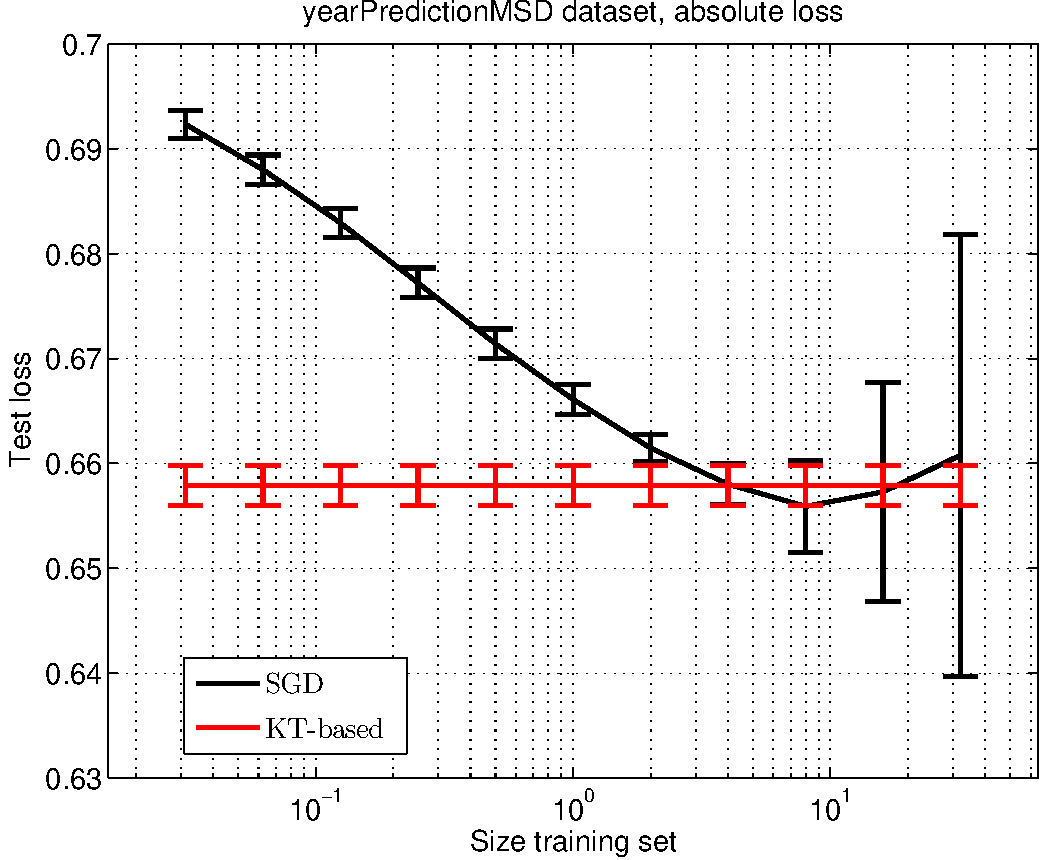
\includegraphics[width=0.32\textwidth]{figs/yearPredictionMSD_kt_train_test-crop.pdf}}
\subfigure{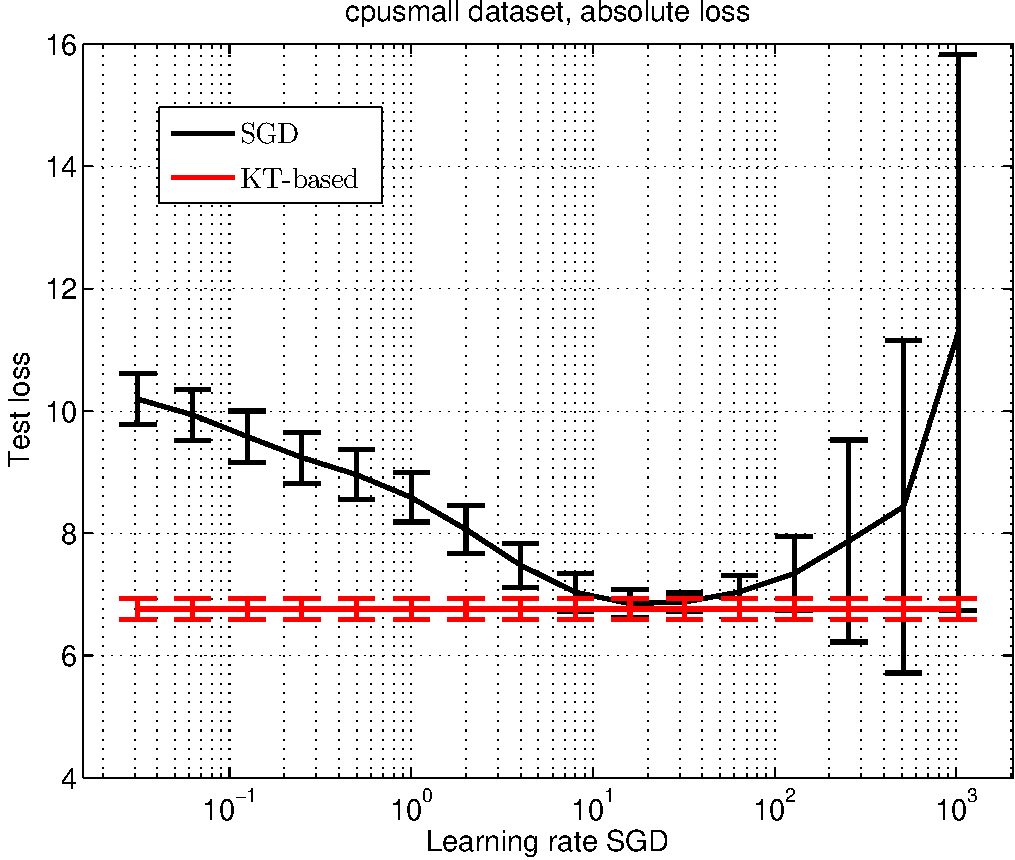
\includegraphics[width=0.32\textwidth]{figs/cpusmall_kt_train_test-crop.pdf}}
\subfigure{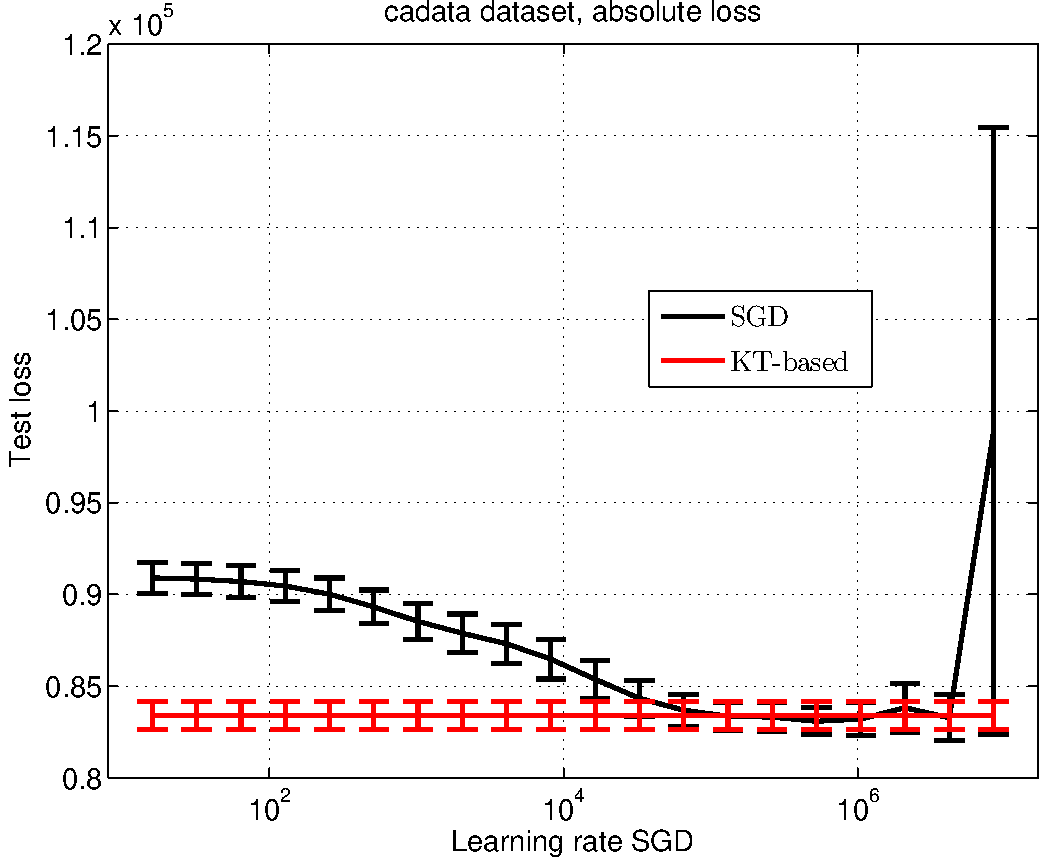
\includegraphics[width=0.32\textwidth]{figs/cadata_kt_train_test-crop.pdf}}
\caption{\footnotesize{Test loss versus learning rate parameter of \ac{SGD} (in log scale), compared with the parameter-free Algorithm~\ref{algorithm:averaged-olo}.}}
\label{figure:experiments-olo}
\end{figure}

We have also run a small empirical evaluation to show that the theoretical
difference between classic learning algorithms and parameter-free ones is real
and not just theoretical. In Figure~\ref{figure:experiments-olo}, we have used
three regression datasets\footnote{Datasets available at
\url{https://www.csie.ntu.edu.tw/~cjlin/libsvmtools/datasets/}.}, and solved
the \ac{OCO} problem through \ac{OLO}. In all the three cases, we have used the
absolute loss and normalized the input vectors to have L2 norm equal to 1. 

The dataset were split in two parts: 75\% training set and the remaining as test set. The training is done through one pass over the training set and the final classifier is evaluated on the test set. We used 5 different splits of training/test and we report average and standard deviations. 

We have run \ac{SGD} with different learning rates and shown the performance of its last solution on the test set. For Algorithm~\ref{algorithm:averaged-olo}, we do not have any parameter to tune, we just plot its test set performance.

From the empirical results, it is clear that the optimal learning rate is completely
data-dependent, yet \emph{our parameter-free algorithm has a performance very close
to the unknown optimal tuning of the learning rate of \ac{SGD}}.


\newpage

% Acknowledgments---Will not appear in anonymized version
\acks{The authors thank Jacob Abernethy, Nicol\`{o} Cesa-Bianchi, Satyen Kale, Chansoo Lee, and Giuseppe Molteni for useful discussions on this work.}

\bibliography{learning}

\end{document}
